\begin{enumerate}[label=\thesection.\arabic*.,ref=\thesection.\theenumi]
\numberwithin{equation}{enumi}
\item A unity negative feedback system has the open loop transfer function 
\begin{align}
    G(s) = \frac{K}{s(s+1)(s+3)} 
    \label{eq:ee18btech11050_t1}
\end{align}
Find the value of the gain K ($>$0) at which the root locus crosses the imaginary axis.

\solution From     \label{eq:ee18btech11050_t1}, the characteristic function of the control system is 
    \begin{align}
        s^3 + 4s^2 + 3s + K = 0
    \end{align}
%
If all elements of any row of the Routh array table are zero, then the root locus branch intersects the imaginary axis.  The Routh array is
    \begin{align}
        \mydet{s^3\\s^2\\s^1\\s^0}
&        \mydet{1 & 3\\ 4 & K \\ (12-K)/4 & 0 \\ K}
\\
  \implies       \frac{12-K}{4} &= 0
\\
\text{or, }K &= 12.
\end{align}

The following code plots the root locus in Fig. \ref{eq:ee18btech11050}

\begin{lstlisting}
codes/ee18btech11050.py
\end{lstlisting}    

\item Root Locus plot
    \begin{figure}[!h]
\centering
        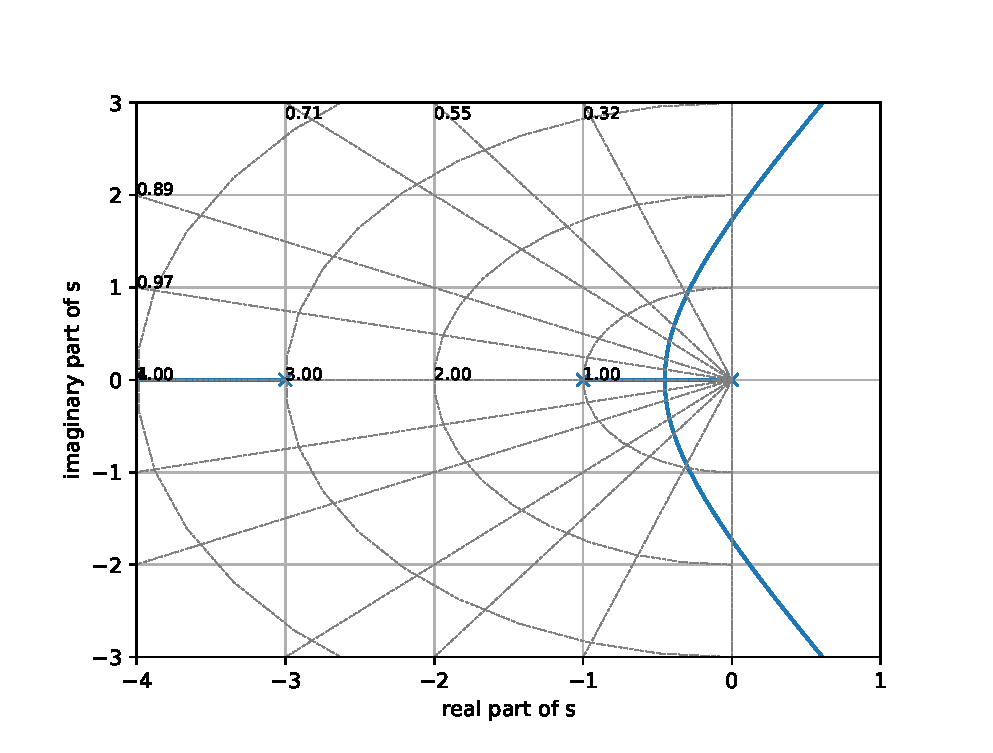
\includegraphics[width=\columnwidth]{./figs/ee18btech11050.eps}
\caption{}
\label{eq:ee18btech11050}
    \end{figure}
	

\end{enumerate}
